% Appendix A
\chapter{Implementing Dynamic Energy Map in
  CityEngine} % Main appendix title

\label{AppendixA} % For referencing this appendix elsewhere, use
                  % \ref{AppendixA}

\lhead{Appendix A. \emph{Implementing Dynamic Energy Map in CityEngine}} % This is for the header on each page - perhaps a shortened title
\section{General Introduction}
The following document records the method of using CityEngine to
visualize the dynamic energy (heating energy in kwh for this document)
changes with a slider bar embeded in the CityEngine software. To be
more specific, users will be able to navigate through the 8760 hour of
a year with a time slider and see the color-coded energy consumption
data for all buildings in the community model for the hour the slider
cursor rest at. The detailed rule file is included in \aref{AppendixB}.

The general process is to find a base map if it is a real site or
generate a random urban environment layout if it is a conceptual
setting. Add attributes of ``landuse'' and ``time'' to the building
lot. Then write a rule file with energy consumption data (or the color
representation of each energy consumption data) for each building type
held in string lists in the rule file and then apply the rule files to
the building lot. Finally set the attribute of ``landuse'' and
``time'' in the rule file to be driven by the value of the object
attribute ``landuse'' and ``time''. The ``time'' attribute is to index
into the string list of energy profile (in rule files) for each
building type. For example, when the ``time'' attribute of all building
blocks are set to 10, all the buildings in the community model will
change its color to the color representing its heating energy
consumption in the 10th hour (zero-indexing) of the year.

Each step will be explained in more details in the following session.
\section{Explaining Each Steps}
\begin{enumerate}[1)]
\item{Create a Urban Environment Layout}

  If one is working with a real project, an OSM Map~\cite{OSM2015}
  will be a good choice for a base map. The OSM file contains many
  useful attribute such as street center line, building name,
  elevation etc. It is of xml format and is easy to manipulate as text
  files, which makes it easier to work with and less bulky comparing
  to ArcGIS gdb files. \fref{fig:osmCampus} is an example of the CMU
  Campus OSM Map.

  \begin{figure}[h!]
    \centering
    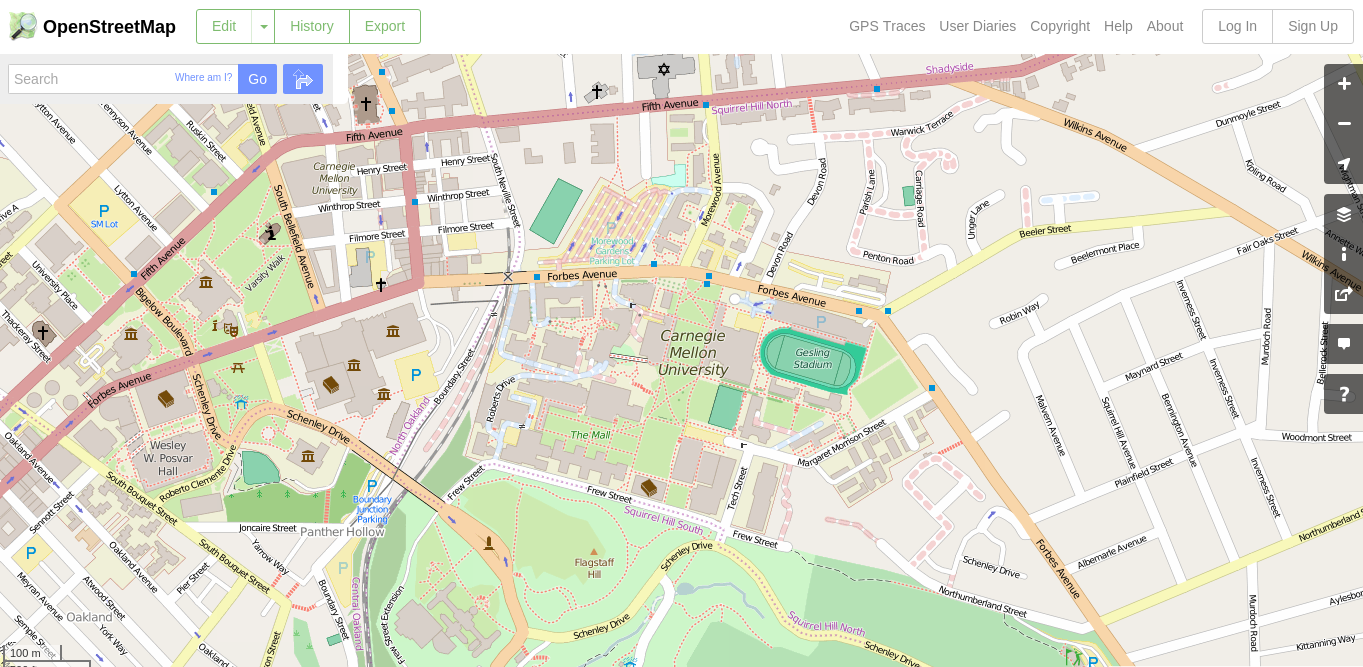
\includegraphics[width=0.7\linewidth]{osmCampus.png}
    \caption[CMU OSM Map]{CMU OSM Map~\cite{OSM2015}}
    \label{fig:osmCampus}
  \end{figure}

  If it is a conceptual setting, then create a random city of proper
  size using ``grow street'' function with some clean-ups
  (\fref{fig:randCity}).

  \begin{figure}[h!]
    \centering
    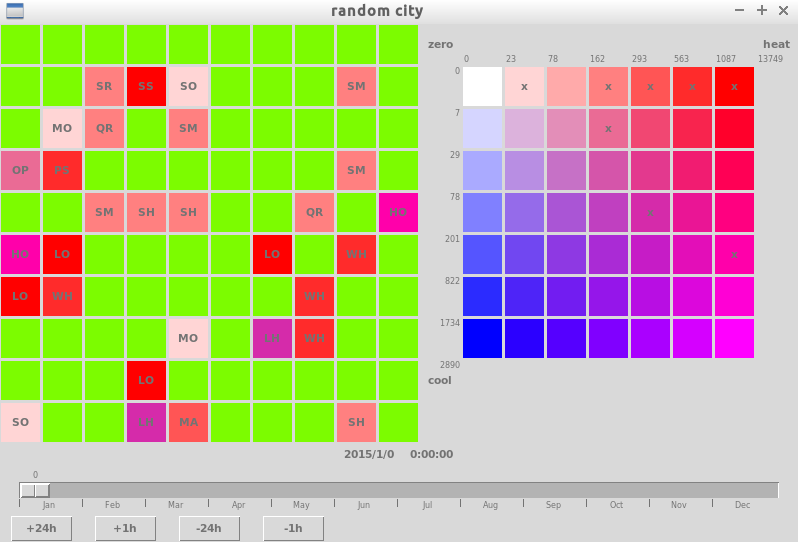
\includegraphics[width=0.7\linewidth]{randCity.png}
    \caption[Conceptual City Lots]{Conceptual City Generated with
      CityEngine}
    \label{fig:randCity}
  \end{figure}

\item{Add Attributes to Building Lots} 

  To implement the function of a time slider-bar that navigates and
  shows energy consumption for each building in each hour of the year,
  two additional attributes are needed: 1) ``time'' attribute of type
  float (ideally we would like it to be integer but there is no
  integer types in object attribute) ranges from 0 to 8760 (not
  inclusive) that represents the hour of a year and 2) ``landuse''
  attribute of type float (since no integer type is available) that
  represents the land use type of the lot.

  Adding these two attribute could be done either inside an OSM base
  map or inside CityEngine.

  The typical way to add a building attribute can be done by selecting
  all building lots and right click one of the Object attributes and
  select "Add Object Attribute" to add new attributes.

  If an OSM base map is available with building footprint information,
  adding attributes can be achieved within OSM maps by one searching
  for \texttt{"<tag k="building" v="yes"/>"} and add two new tags
  after this
  line:\\
  \texttt{"<tag k="time" v="0"\/>"}\\
  \texttt{"<tag k="landuse" v="0"\/>"}\\

\item{Importing Base Map (Optional)}

  If one is working on a real project, one can add an geo-referenced
  terrain image to make the model more realistic. In the following
  example, the terrain geo-tiff was retieved from PASDA
  website~\cite{PASDAImagery2013} according to the ``Allegheny County
  Imagery 2013 - Tile Index''. The image showing the area of interest
  is clipped in ArcMap and imported as a geo-referenced image (.tif)
  to CityEngine (\fref{fig:geotif}).

  \begin{figure}[h!]
    \centering
    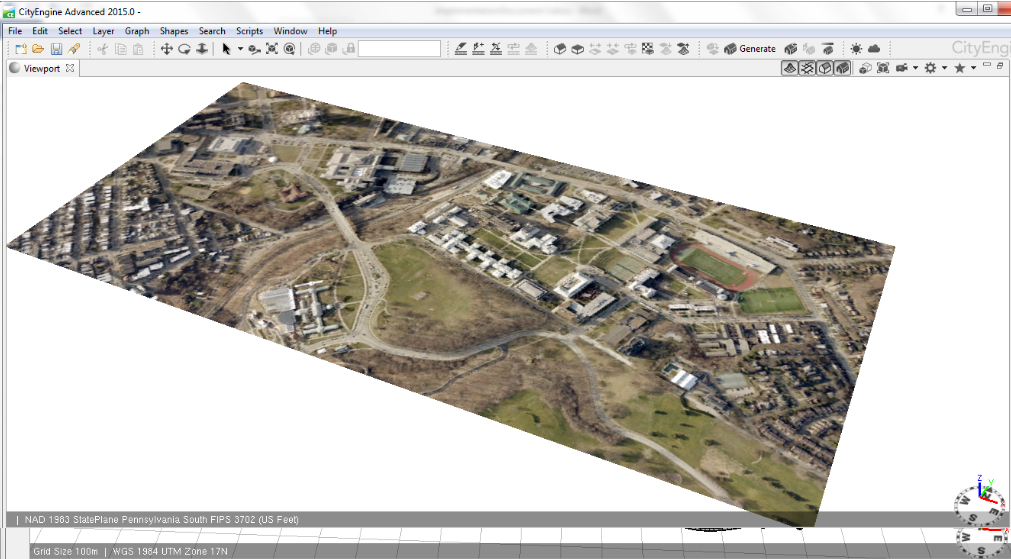
\includegraphics[width=0.7\linewidth]{geotif.png}
    \caption[Geo-tif in CityEngine]{Example of Geo-referenced Image in
      CityEngine}
    \label{fig:geotif}
  \end{figure}

  After importing geo-referenced image, OSM map could be imported and
  a working base was formed (\fref{fig:geotifOSM}).
  \begin{figure}[h!]
    \centering
    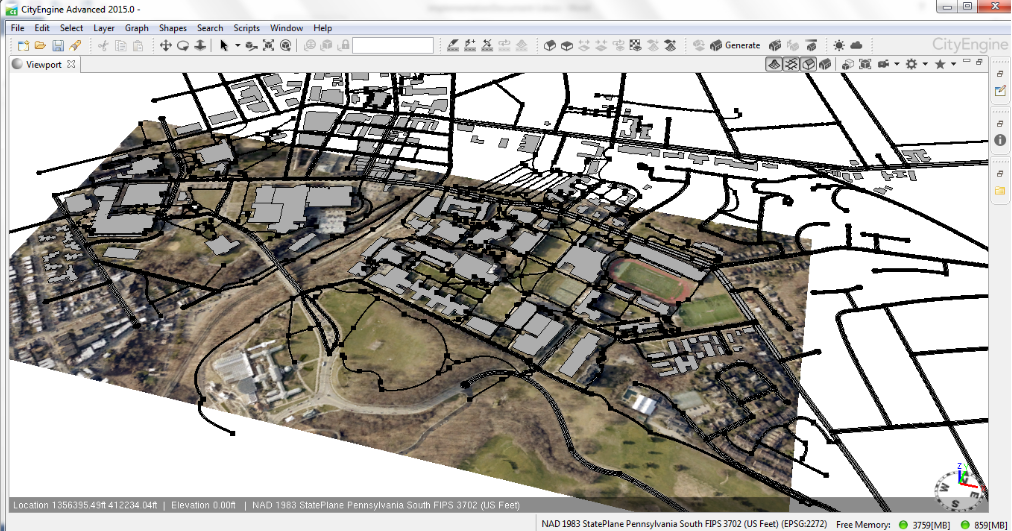
\includegraphics[width=0.7\linewidth]{geotifOSM.png}
    \caption[Geo-tif with OSM Map]{Geo-tif with OSM Map}
    \label{fig:geotifOSM}
  \end{figure}

\item{Writing Rule File for Building Generation}

  We used ``time'' as the index into the string array that holds the
  hourly heating energy consumption data. By setting the rule
  attribute ``time'' to some $t$, we will be able to retrieve the
  energy consumption information at hour ``$t$'' from the energy
  string list.

  When implementing the dynamic energy map inside CityEngine, one
  should decide a proper color scheme for encoding the energy
  consumption data. No building-science specific breakpoints were
  specified at the current stage of the project. We used the continues
  red-to-blue color ramp in the stand-alone CityEngine based Dynamic
  Energy Map implementation.

\item{Deciding Data Encoding}

  The first approach for representing energy information with color is
  to encode it with a graduated color symbol from red to blue, with
  red indicating low heating demand and blue indicating high heating
  demand. Each color within this red-to-blue color scheme is
  represented as a real number between 0 and 1 with 0 representing
  pure red and 1 representing pure blue. The first approach to
  calculate the corresponding color for each heating energy value is
  to calculate the normalized distance between the current value and
  the maximum value (\eref{eq:linear}).

  \begin{equation}\label{eq:linear} 
    {E_{current} – E_{max} \over E_{max}}
  \end{equation}

  $E_{current}$ is the energy consumption for the current time spot,
  $E_{max}$ is the maximum energy consumption over the year. The
  problem for this approach is that the color changing is not visible
  enough as a result of a extremely right skewed energy data (with
  each data point representing the hourly energy consumption of a
  certain building in the community at a certain hour of a year)
  distribution (\fref{fig:heatOri}).

  \begin{figure}[h!]
    \centering
    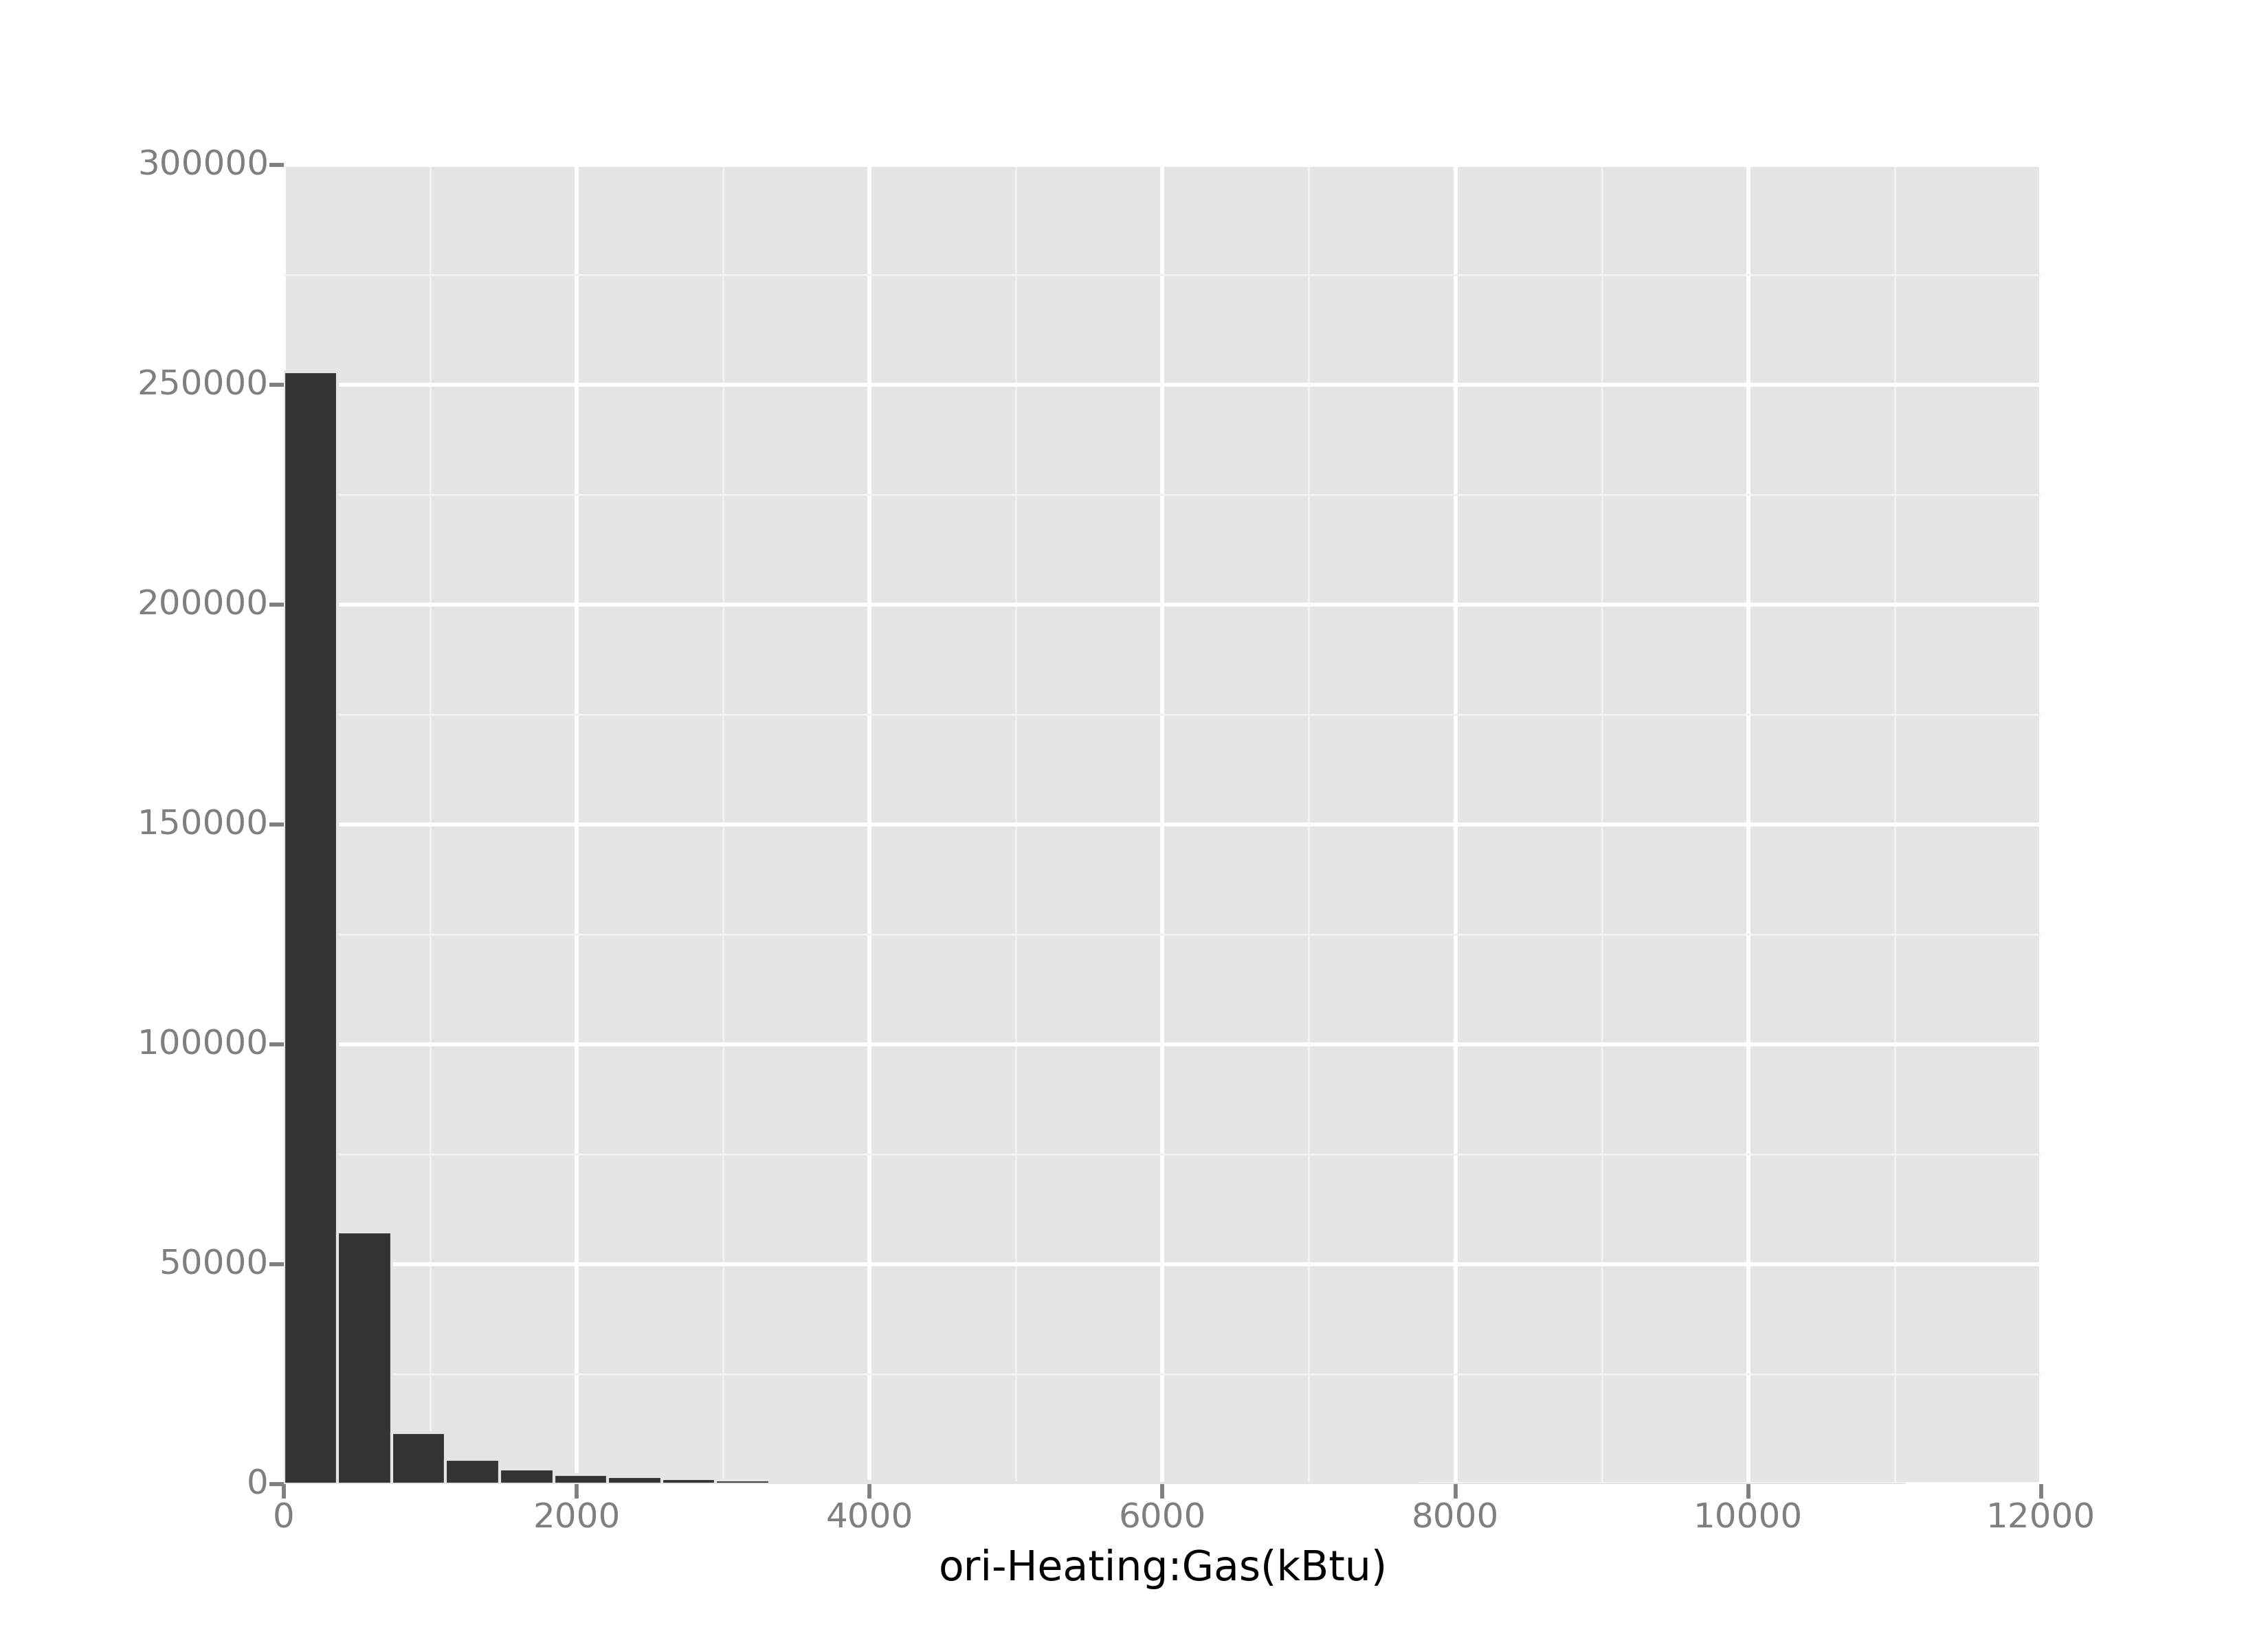
\includegraphics[width=0.7\linewidth]{heatOri.png}
    \caption[Heating Demand Histogram of Conceptual City]{A histogram
      of hourly energy consumption per building, for the 68 buildings
      in the community}
    \label{fig:heatOri}
  \end{figure}

  By directly applying this normalized color scheme, the color
  distribution on a map will be very un-even, with most of the
  buildings colored with the red color for most of the time.

  Kolter and Ferreira has used discovered that the annual total energy
  consumption of the 6500 buildings in Cambridge MA area follows a
  ``log-normal'' distribution~\cite{Zico2011}. By applying similar log
  scaling for the hourly heating energy data of the community, we
  found that the hourly heating energy distribution also roughly
  follows a normal distribution (\fref{fig:heatLog}). We apply log
  scaling to make the distribution less skewed and calculate the color
  from energy ($E_{current}$) as follows:

  \begin{equation}\label{eq:log} 
    {\ln(E_{current}) – \ln(E_{max}) \over \ln(E_{max})}
  \end{equation}

  \begin{figure}[h!]
    \centering
    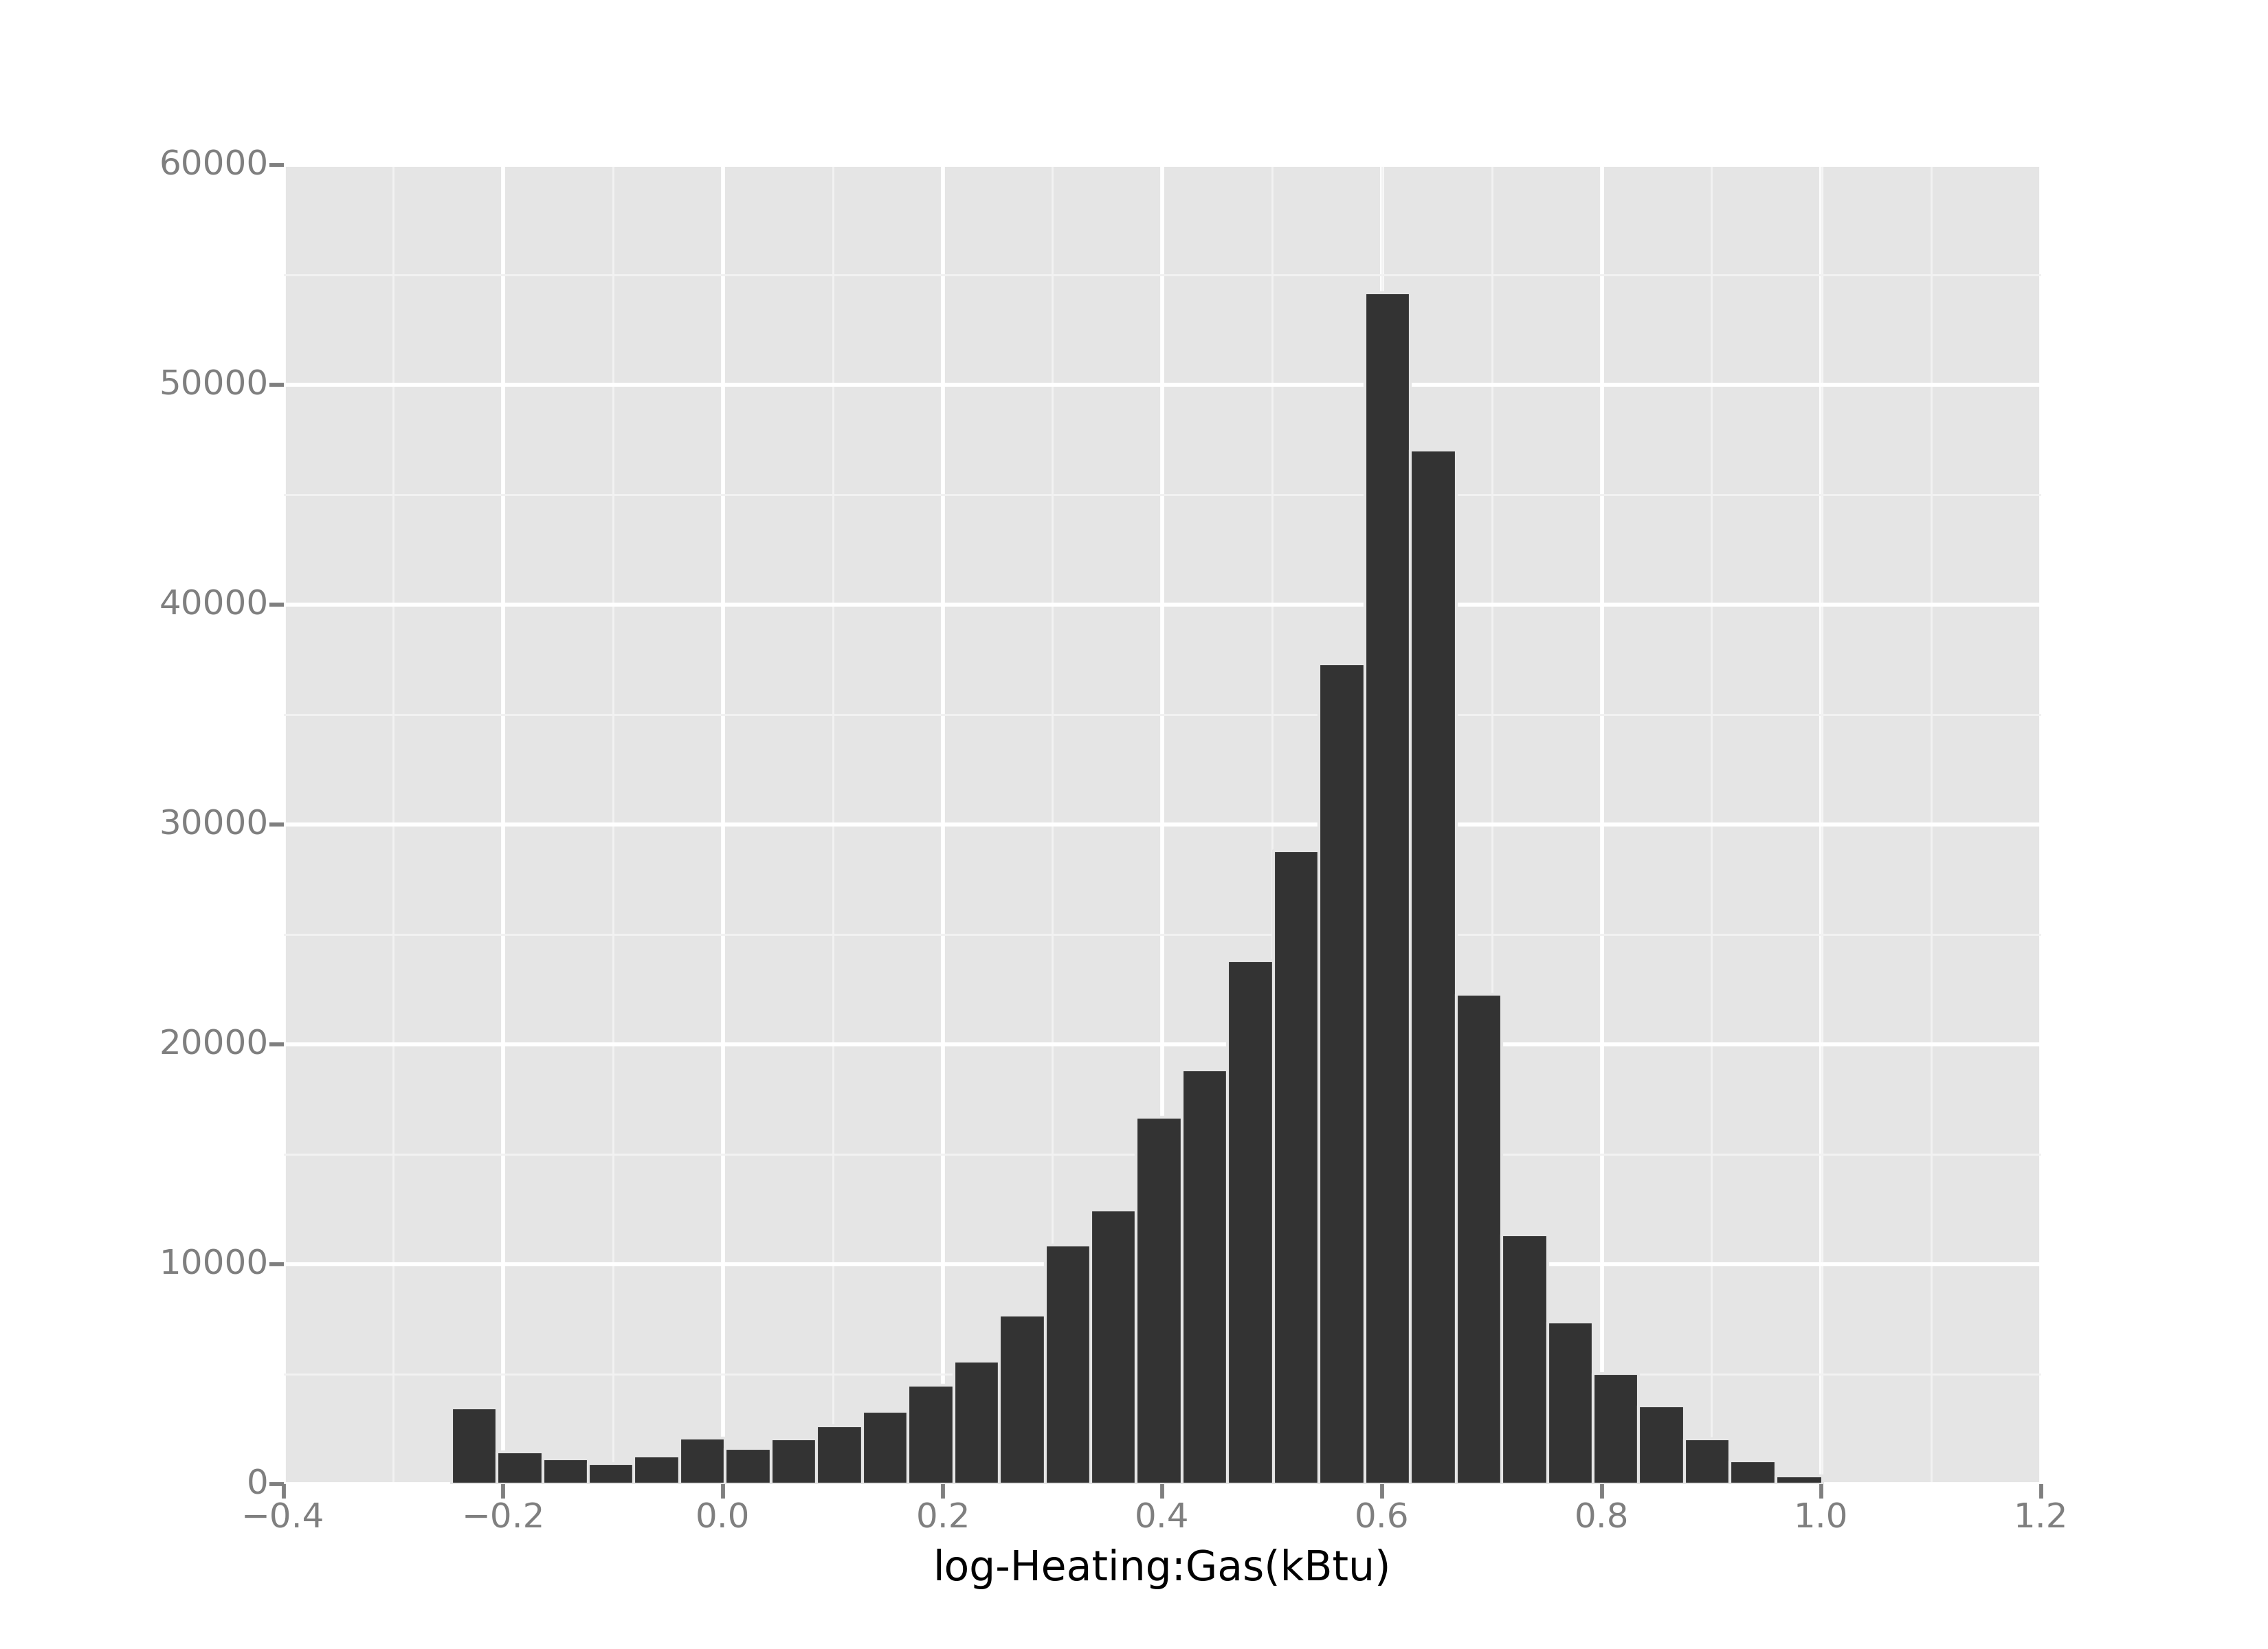
\includegraphics[width=0.7\linewidth]{heatLog.png}
    \caption[Heating Demand of Conceptual City]{Heating Demand of
      Conceptual City}
    \label{fig:heatLog}
  \end{figure}

  \fref{fig:img0002} is one snapshot of the conceptual urban
  environment model under the log scaled calculation method in
  \eref{eq:log}.
  \begin{figure}[h!]
    \centering
    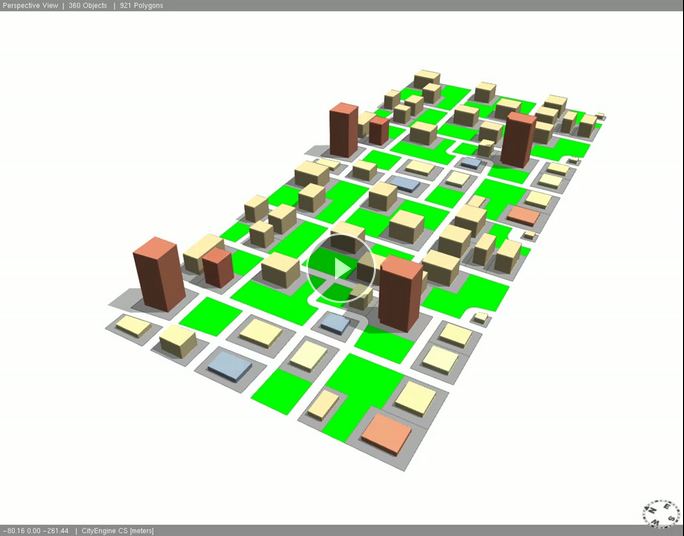
\includegraphics[width=0.7\linewidth]{img0002.png}
    \caption[Animation Demo of the Color Calculation]{Animated
      demonstration of the log-scaled dynamic energy heating demand
      map}
    \label{fig:img0002}
    \href{http://www.armechxyj.com/energy-mapping.html/#colorAnime}{Click
      here to go to the animation link}.
  \end{figure}

\item{Associating Rule Attribute with Object Attribute} 

  How to globally set all ``time'' attribute for each rule file is a
  key problem to solve to implement the time-navigation. Writing a
  python code for processing all the rule files as pure text files and
  apply rule files to its corresponding lot at each given ``time''
  could be one solution, but there are two drawbacks 1) it is time and
  space consuming because as many as each 8760 rule files need to be
  generated 2) the ``slider-bar'' feature associated with the object
  attribute will not be available if implemented this way.

  We want to use object attribute (building lot) to drive the change
  of ``time'' for rule files for each building. The way to create the
  connection between object attribute ``time'' and the building
  attribute defined in rule files is by setting the source of ``time''
  attribute (in rule file) by the building lot ``time'' attribute
  using ``Connection Editor''~\cite{cityEngineAttConect2015}.

  After the connection is established, one will select all buildings
  of interest in the community model and change the object attribute
  ``time'' of all selected building lots to visually inspect the
  color-coded energy consumption of all selected buildings. The Campus
  example is depicted in \fref{fig:timeSliderCampus} and the community
  example is depicted in (Add figure here !!!)

  \begin{figure}[h!]
    \centering
    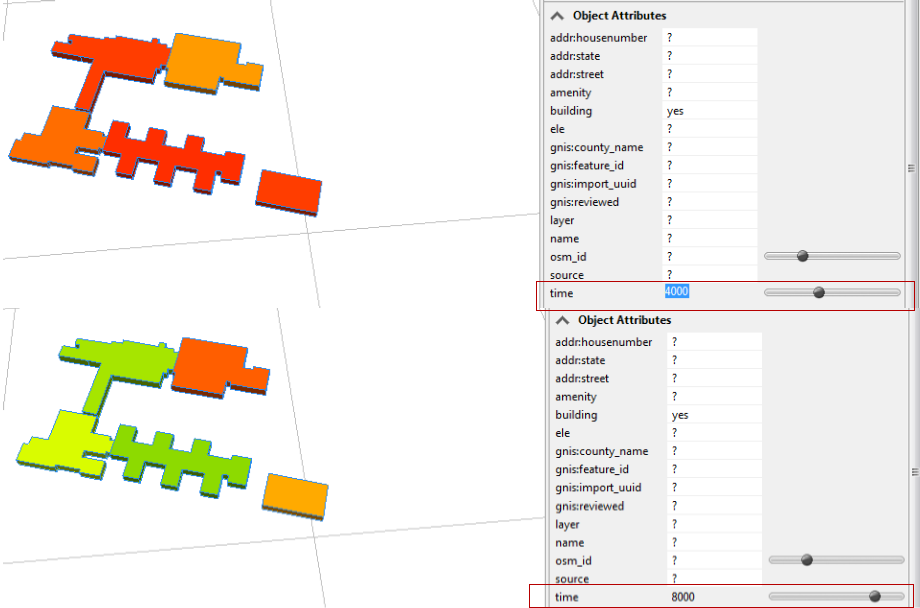
\includegraphics[width=0.7\linewidth]{timeSliderCampus.png}
    \caption[Slider in Campus Example]{Slider in Campus Example}
    \label{fig:timeSliderCampus}
  \end{figure}
  \begin{figure}[h!]
    \centering
    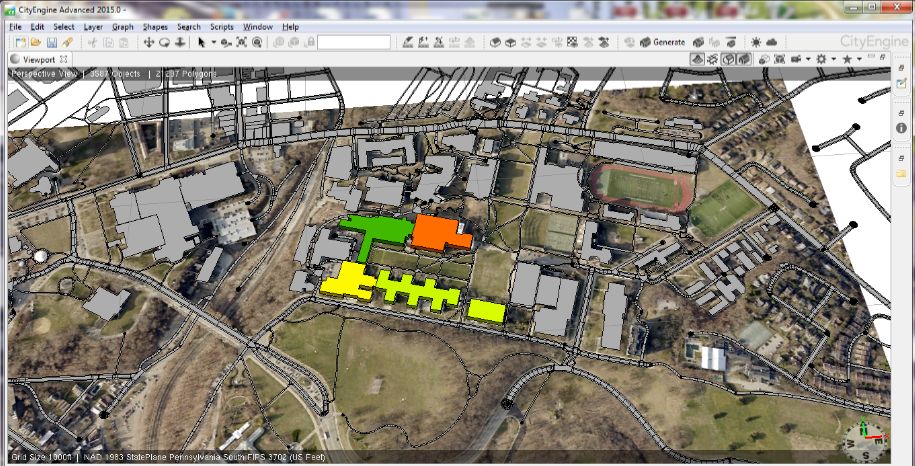
\includegraphics[width=0.7\linewidth]{campusColor.png}
    \caption[Finished Campus Example]{Finished Campus Example}
    \label{fig:campusColor}
  \end{figure}

  \begin{figure}[h!]
    \centering
    \begin{subfigure}{0.7\textwidth}
      \centering
      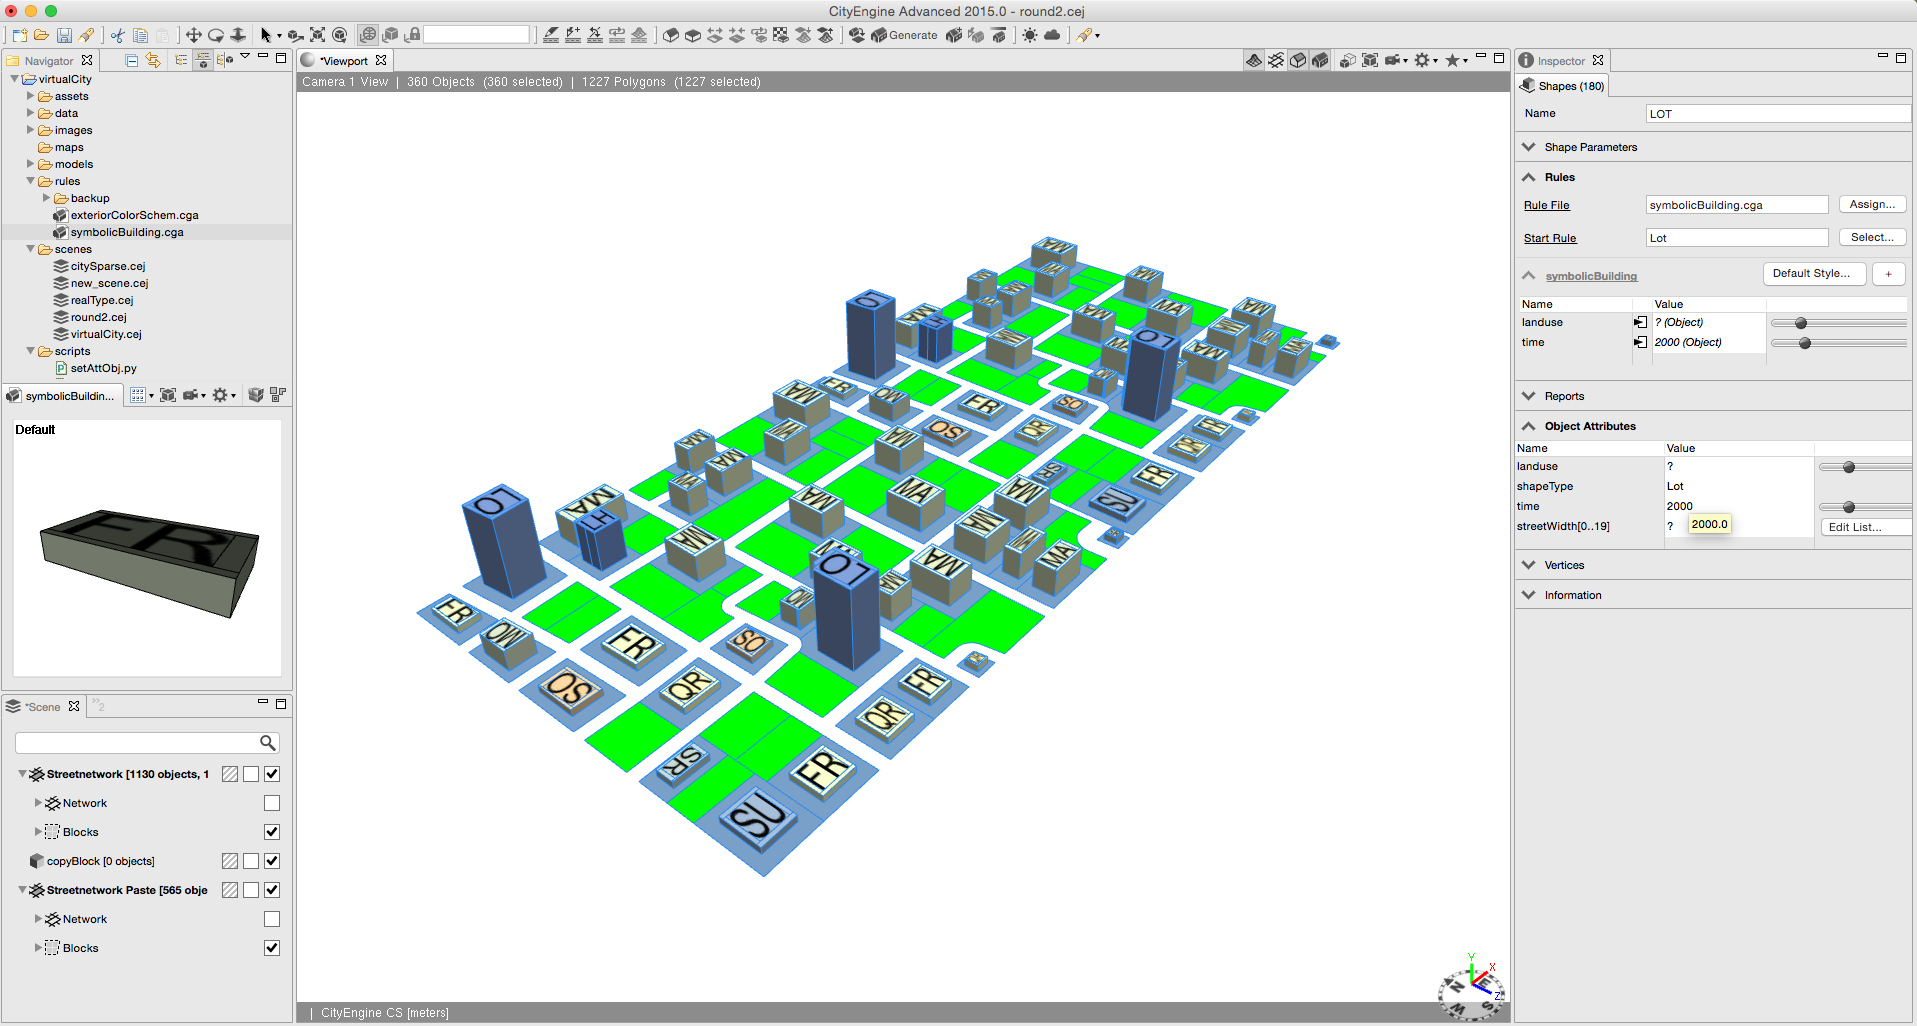
\includegraphics[width=\linewidth]{sliderImag.png}
      \caption[Conceptual Community Setting Slider Winter]{Conceptual
        Community Setting Slider Winter}
      \label{fig:sliderImag}
    \end{subfigure}
    ~
    \begin{subfigure}{0.7\textwidth}
      \centering
      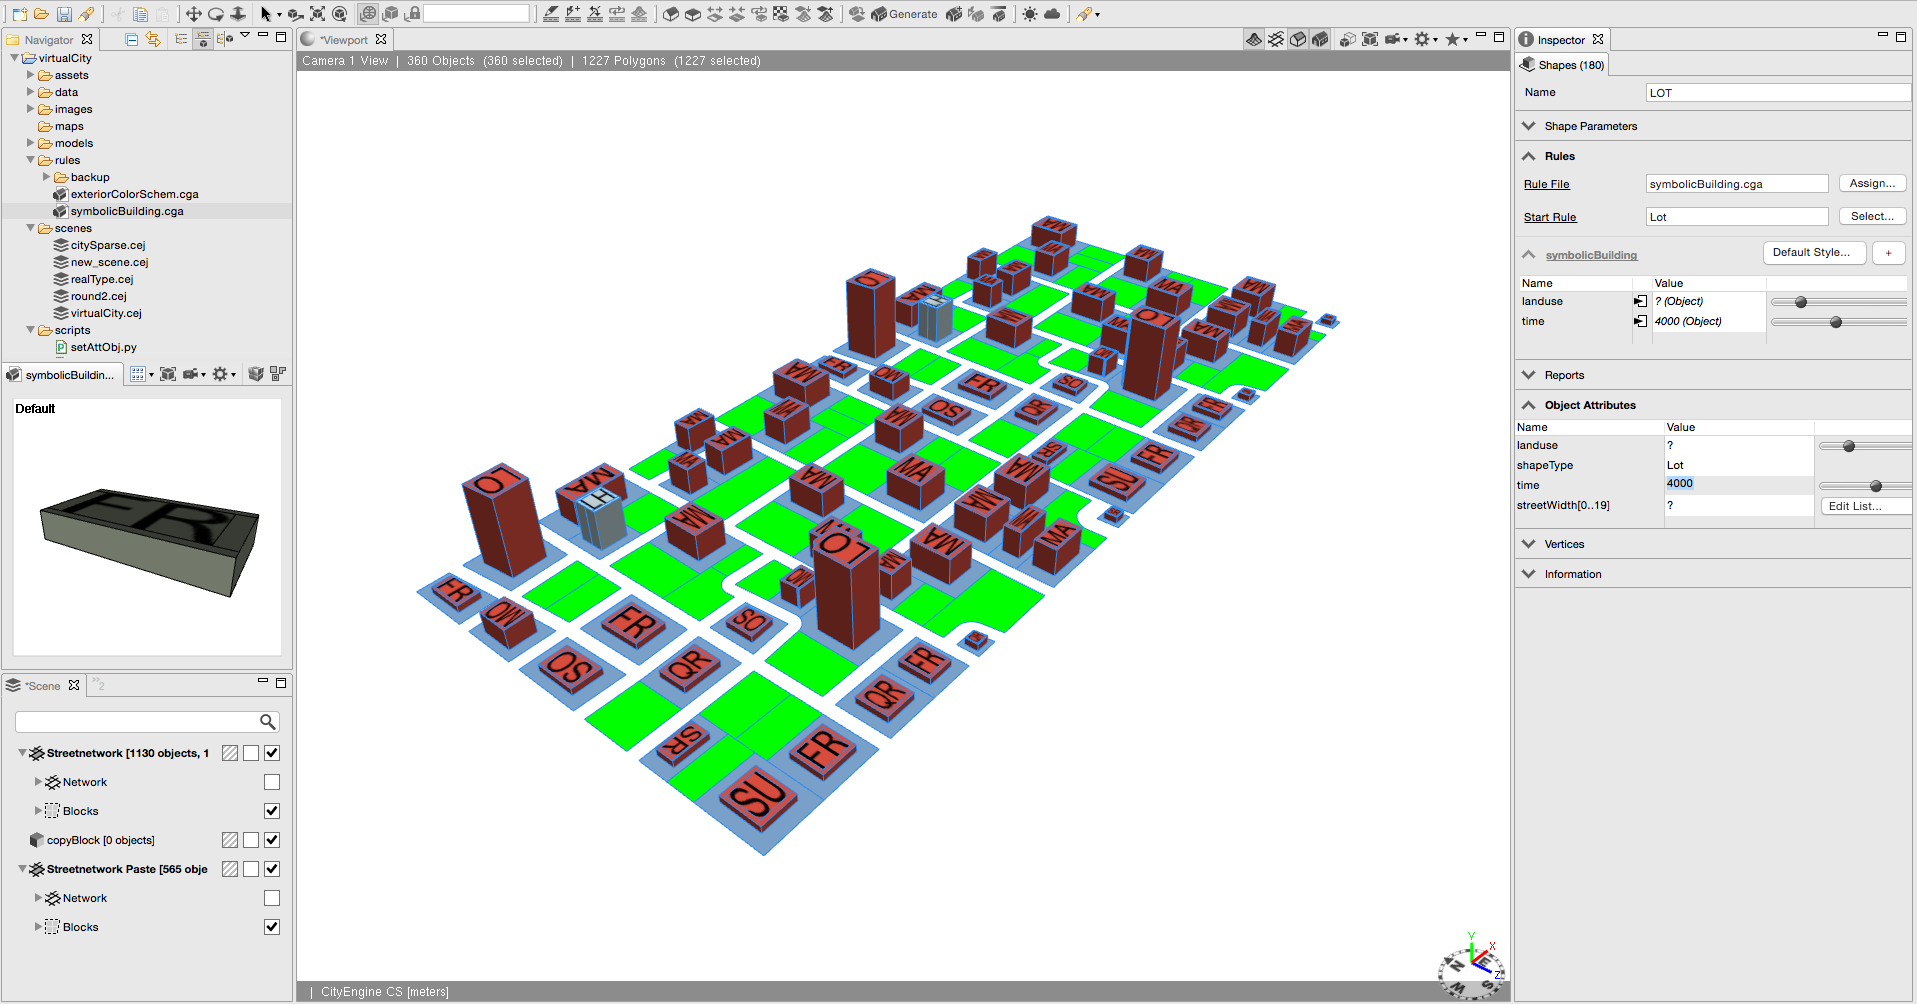
\includegraphics[width=\linewidth]{sliderImag2.png}
      \caption[Conceptual Community Setting Slider Summer]{Conceptual
        Community Setting Slider Summer}
      \label{fig:sliderImag2}
    \end{subfigure}
  \end{figure}

\item{Sharing the Map}

  This is not achievable with CityEngine itself. The sharing of
  CityEngine models is through publishing a ``web scene'' or through
  sharing a ``rule package''. The first approach only shares the
  building geometry, not the building lots and the building lot
  attribute function. Since the dynamic map operates on setting the
  building lot object attribute, when shared with publishing ``web
  scene'', the temporal dimension is lost. The other approach is
  through sharing the ``rule package'', since the building energy
  demand data are included in the rule file, by sharing the model and
  the rule package, all functions of the dynamic energy map one
  implemented inside CityEngine can be retained. The drawback is that
  it requires the views of the dynamic energy map 1) having CityEngine
  software, which is not free 2) having sufficient knowledge of the
  CityEngine software.

  Another way to share the dynamic map implemented in this way is
  through a streamed animation or video. More details on animated maps
  will be explained in a separate section X. Here only the procedure
  is presented.
\end{enumerate}